\documentclass{ltjsarticle}
\RequirePackage{luatex85}
\usepackage[utf8]{inputenc}
\usepackage[dvipdfmx]{color}
\usepackage{enumerate}
\usepackage{here}
\usepackage{amsthm}
\usepackage{amsfonts}
\usepackage{amsmath}
\usepackage{amssymb}
\usepackage{latexsym}
\usepackage{ytableau}
\usepackage{docmute}
\usepackage{mathtools}
\usepackage{xr}
\usepackage{tikz}
\usetikzlibrary{intersections, calc, arrows.meta}
\usepackage[all]{xy}
\usepackage{graphics}
\usepackage[luatex]{hyperref}
%\usepackage{pxjahyper}



\theoremstyle{definition}
\newtheorem{defin}{定義}[subsection]
\newtheorem{theo}[defin]{定理}
\newtheorem{cor}[defin]{系}
\newtheorem{prop}[defin]{命題}
\newtheorem{lemm}[defin]{補題}
\newtheorem{notice}[defin]{注意}
\newtheorem{eg}[defin]{例}
\newtheorem{fact}[defin]{事実}


\renewcommand{\labelenumi}{(\roman{enumi})}


\newcommand{\invlimit}{\mathop{\lim_{\longleftarrow}}}
\newcommand{\dirlimit}{\mathop{\lim_{\longrightarrow}}}
\newcommand{\ind}{\text{Ind}}
\newcommand{\Hom}{\text{Hom}}
\newcommand{\tr}{\text{tr}}
\newcommand{\id}[1]{\text{id}_{#1}}
\newcommand{\sgn}{\mathrm{sgn}}
\newcommand{\res}[1]{\text{Res}_{#1}}
\newcommand{\generated}[1]{\langle\:#1\:\rangle}
\newcommand{\im}{\text{Im }}
\newcommand{\rank}{\text{rank }}
\newcommand{\del}[2]{\frac{\partial #1}{\partial #2}}
\newcommand{\delsametwo}[2]{\frac{\partial^2 #1}{\partial #2^2}}
\newcommand{\delothertwo}[3]{\frac{\partial^2#1}{\partial#2\partial#3}}
\newcommand{\ddel}[2]{\frac{\partial}{\partial #2}#1}
\newcommand{\ddelsametwo}[3]{\frac{\partial^2}{\partial #2^2}#1}
\newcommand{\ddelothertwo}[3]{\frac{\partial^2}{\partial#2\partial#3}#1}
\newcommand{\simneq}{\not\simeq}
\newcommand{\transpose}[1]{^t\!#1}
\newcommand{\ie}{\text{i.e.}}
\newcommand{\inv}[1]{#1^{-1}}
\newcommand{\real}{\mathbb{R}}
\newcommand{\complex}{\mathbb{C}}
\newcommand{\integer}{\mathbb{Z}}
\newcommand{\quotient}{\mathbb{Q}}
\newcommand{\natnum}{\mathbb{N}}
\newcommand{\proj}{\mathbb{P}}
\newcommand{\affine}{\mathbb{A}}
\newcommand{\tensor}[3]{#1\otimes_#2#3}
\newcommand{\map}[3]{#1:#2\rightarrow#3}
\newcommand{\aut}[2]{\mathrm{Aut}_{#1} (#2)}
\newcommand{\hommoph}[2]{\mathrm{Hom}_{#1}(#2)}
\newcommand{\gl}{\text{GL}}
\newcommand{\End}{\text{End}}
\newcommand{\set}[2]{\left\{\:#1\:\middle|\:#2\:\right\}}
\newcommand{\pmat}[1]{\begin{pmatrix} #1
\end{pmatrix}}
\newcommand{\vmat}[1]{\begin{vmatrix} #1
\end{vmatrix}}
\newcommand{\bmat}[1]{\begin{bmatrix} #1
\end{bmatrix}}
\newcommand{\br}{\vskip\baselineskip}
\newcommand{\Lie}{\text{Lie}}
\newcommand{\Sym}{\text{Sym}}
\newcommand{\Alt}{\text{Alt}}
\newcommand{\ch}{\text{ch}}
\newcommand{\diag}{\text{diag}}
\newcommand{\comb}[2]{_{#1}C_{#2}}
\newcommand{\codim}{\text{codim}\:}
\newcommand{\yd}[1]{\ydiagram{#1}}

\title{aaa}
\author{}
\date{}


\begin{document}
\maketitle

\begin{figure}[H]
  \centering
  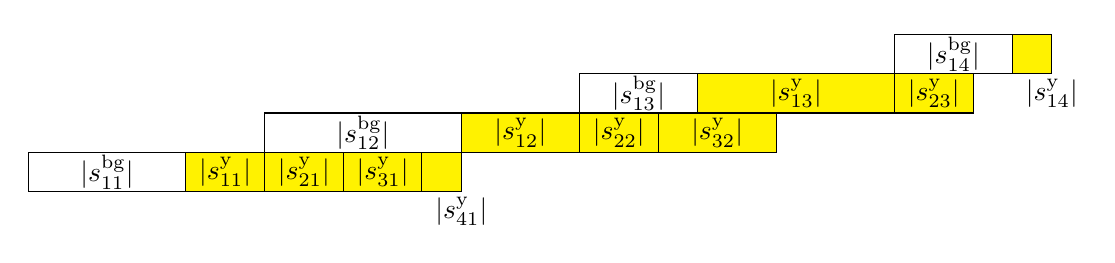
\begin{tikzpicture}
    \draw (0,0) rectangle ++(2,1/2);
    \node at (1,1/4) {$|s_{11}^{\text{bg}}|$};
    \filldraw[fill=yellow] (2,0) rectangle ++(1,1/2);
    \node at (2.5,1/4) {$|s_{11}^{\text{y}}|$};
    \filldraw[fill=yellow] (3,0) rectangle ++(1,1/2);
    \node at (3.5,1/4) {$|s_{21}^{\text{y}}|$};
    \filldraw[fill=yellow] (4,0) rectangle ++(1,1/2);
    \node at (4.5,1/4) {$|s_{31}^{\text{y}}|$};
    \filldraw[fill=yellow] (5,0) rectangle ++(1/2,1/2);
    \node at (5.5,-0.25) {$|s_{41}^{\text{y}}|$};

    \draw (3,1/2) rectangle ++(5/2,1/2);
    \node at (8/2+1/4,3/4) {$|s_{12}^{\text{bg}}|$};
    \filldraw[fill=yellow] (11/2, 1/2) rectangle ++(3/2,1/2);
    \node at (12/2+1/4,3/4) {$|s_{12}^{\text{y}}|$};
    \filldraw[fill=yellow] (14/2, 1/2) rectangle ++(2/2,1/2);
    \node at (15/2,3/4) {$|s_{22}^{\text{y}}|$};
    \filldraw[fill=yellow] (16/2, 1/2) rectangle ++(3/2,1/2);
    \node at (17/2+1/4,3/4) {$|s_{32}^{\text{y}}|$};

    \draw (14/2,1) rectangle ++(3/2,1/2);
    \node at (15/2 + 1/4,5/4) {$|s_{13}^{\text{bg}}|$};
    \filldraw[fill=yellow] (17/2,1) rectangle ++(5/2,1/2);
    \node at (19/2 + 1/4, 5/4) {$|s_{13}^{\text{y}}|$};
    \filldraw[fill=yellow] (22/2,1) rectangle ++(2/2,1/2);
    \node at (23/2, 5/4) {$|s_{23}^{\text{y}}|$};

    \draw (22/2,3/2) rectangle ++(3/2,1/2);
    \node at (23/2 + 1/4, 7/4) {$|s_{14}^{\text{bg}}|$};
    \filldraw[fill=yellow] (25/2,3/2) rectangle ++(1/2,1/2);
    \node at (26/2, 5/4) {$|s_{14}^{\text{y}}|$};
  \end{tikzpicture}
  \caption{図\ref{generic puzzle}のpuzzle $P$に対する$\varphi(P)$.黄色のboxにはbox labelが入っており,白いboxにはbox labelは入っていない.}\label{varphi of generic puzzle}
\end{figure}

\end{document}